% ****** Start of file apssamp.tex ******
%
%   This file is part of the APS files in the REVTeX 4.2 distribution.
%   Version 4.2a of REVTeX, December 2014
%
%   Copyright (c) 2014 The American Physical Society.
%
%   See the REVTeX 4 README file for restrictions and more information.
%
% TeX'ing this file requires that you have AMS-LaTeX 2.0 installed
% as well as the rest of the prerequisites for REVTeX 4.2
%
% See the REVTeX 4 README file
% It also requires running BibTeX. The commands are as follows:
%
%  1)  latex apssamp.tex
%  2)  bibtex apssamp
%  3)  latex apssamp.tex
%  4)  latex apssamp.tex
%
\documentclass[%
 reprint,
%superscriptaddress,
%groupedaddress,
%unsortedaddress,
%runinaddress,
%frontmatterverbose, 
%preprint,
%preprintnumbers,
%nofootinbib,
%nobibnotes,
%bibnotes,
 amsmath,amssymb,
 aps,
%pra,
%prb,
%rmp,
%prstab,
%prstper,
%floatfix,
]{revtex4-2}
\usepackage{kotex}
\usepackage{graphicx}% Include figure files
\usepackage{dcolumn}% Align table columns on decimal point
\usepackage{bm}% bold math
\usepackage{chemformula}
\usepackage{setspace,supertabular}
\usepackage{longtable}
\usepackage{multirow}	
\usepackage{makecell}


%\usepackage{hyperref}% add hypertext capabilities
%\usepackage[mathlines]{lineno}% Enable numbering of text and display math
%\linenumbers\relax % Commence numbering lines

%\usepackage[showframe,%Uncomment any one of the following lines to test 
%%scale=0.7, marginratio={1:1, 2:3}, ignoreall,% default settings
%%text={7in,10in},centering,
%%margin=1.5in,
%%total={6.5in,8.75in}, top=1.2in, left=0.9in, includefoot,
%%height=10in,a5paper,hmargin={3cm,0.8in},
%]{geometry}

\begin{document}


\title{MALDI-TOF 펩타이드 질량 분석 결과보고서}

\author{서울대학교 전기정보공학부 2018-12432 박정현}
 \email{alexist@snu.ac.kr}
\date{실험일자: 10/23/2023, 제출일자 : 10/29/2023}% It is always \today, today,
             %  but any date may be explicitly specified

\begin{abstract}
본 실험에서는 MALDI-TOF를 이용해 미지의 단백질의 mass spectrum을 얻은 뒤 hemoglobin, lysozome, BSA, ovalbumin의 amino acid 질량들과 비교 분석하여 어떤 단백질에 해당하는 동정하였다. BSA가 $90\%$의 coverage를 가지고 특정 질량의 amino acid에서 miscleavage가 발생하는 것을 확인하였다. 이를 해결하기 위해 더 긴 시간의 변성시간, 그리고 트립신과의 반응시간이 필요함을 제시하였다.
\end{abstract}

%\keywords{Suggested keywords}%Use showkeys class option if keyword
                              %display desired
\maketitle

%\tableofcontents

\section{\label{sec:level1}Assignment}
\subsection{\label{sec:level2} 1}
\subsubsection{\label{sec:level3} 1}
트립신은 arginie이나 lysine의 carbonyl function에 작용하게 된다. 이로 인해 단백질과 트립신이 작용한 이후에는 Arg, Lys의 C-terminal에서 단백질이 끊어지게 된다.[5]

\begin{figure}[htbp]
	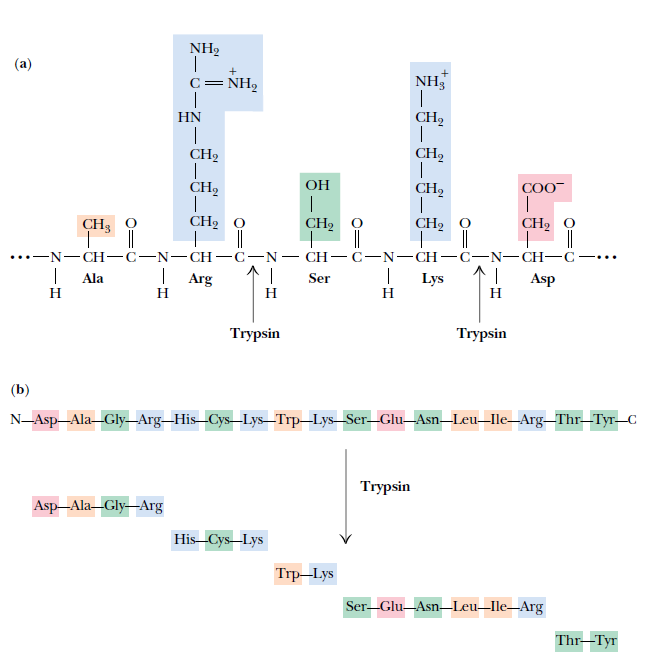
\includegraphics[width = 0.9\linewidth]{trypsin.png}% Here is how to import EPS art
	\caption{\label{fig:trypsin}trypsin의 작용}
\end{figure}

\subsubsection{\label{sec:level3} 2}
키모트립신은 Phenylalanine, Tyrosine, Tryptophan의 카복실 그룹이 만드는 펩타이드 결합을 가수분해한다. 하지만 시간이 지나면 그외의 아미노산을 포함하는 아마이드 결합도 가수분해한다. 더불어서 트립신과 다르게 방향족 아미노산과 잘반응하게 되며 특히 류신이 포함된 가복실기의 펩타이드 결합을 잘 분해한다. 트립신과 키모트립신 모두 catalytic triad에 해당하는 polar residue His57, Asp102, 그리고 Ser195가 움푹 패인 구덩이를 만들어 active site를 만들게 되고 특정 작용기가 해당 구멍에 들어오게 되어 화학 반응이 일어나게 된다. 앞서 말한 catalytic triad는 모두 hydrophobic에 해당한다. Fig.\ref{fig:molecule}와 같이 trypsin은 좁고 깊은 분자 구조 내부에 음전하를 띤 Asp189가 존재하는데 카복실기의 경우 길고 전하를 띠고 있어 이러한 작은 구멍에 잘 들어맞아 반응이 잘 일어나게 된다. 하지만 방향성 분자의 경우 극성을 띠지 않고 크기가 커 구덩이에 들어가지 못해 반응이 일어나기 힘들다. 반면에 키모트립신의 경우 적당한 깊이의 비친수성 구덩이를 만들기 때문에 방향성 분자들이 잘 반응하게 된다. 따라서 트립신과 키모트립신의 분자구조가 달라 작용하는 작용기가 다르기 때문에 각각 다른 단백질을 분해하게 된다.[6]

\begin{figure}[htbp]
	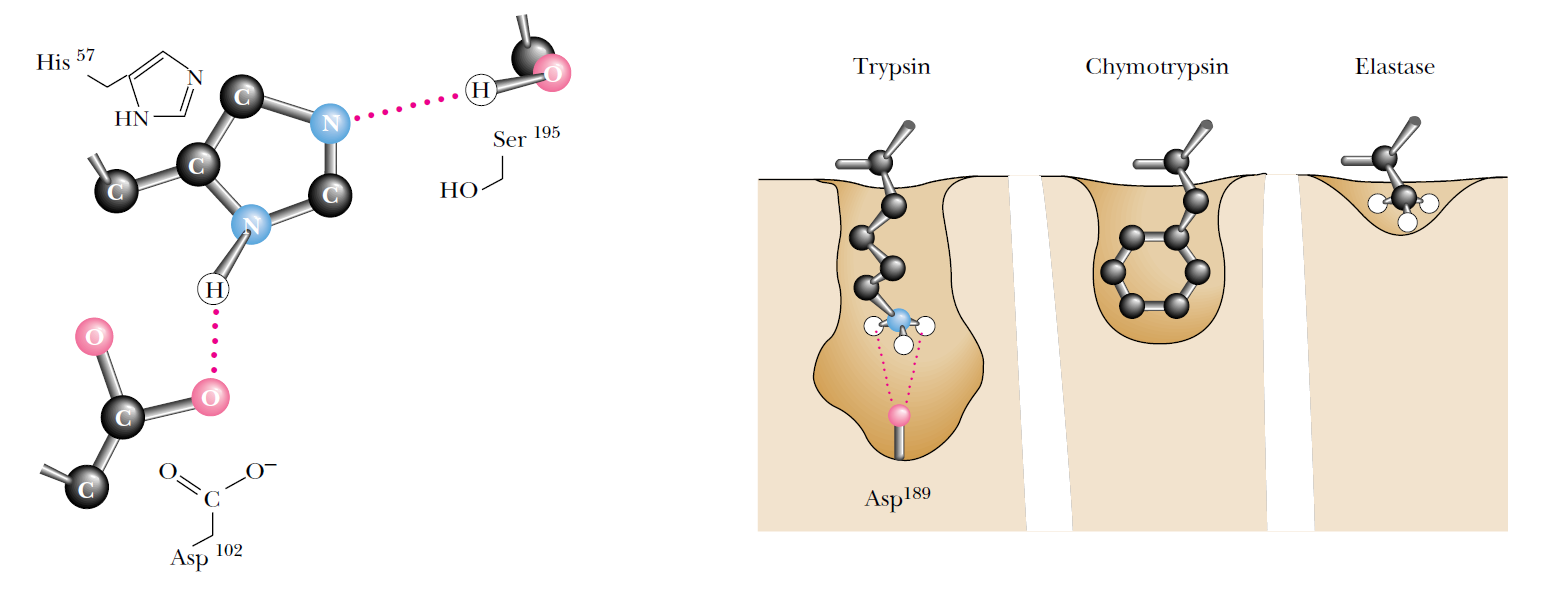
\includegraphics[width = 0.9\linewidth]{molecule.png}% Here is how to import EPS art
	\caption{\label{fig:molecule}트립신과 키모트립신의 분자구조 차이}
\end{figure}

\subsection{\label{sec:level2} 2}
\begin{align}
	\Delta t &= \frac{L}{v}\\
	\frac{1}{2}Mv^{2} &= E\\
	&= \frac{1}{2}M\left( \frac{L}{\Delta t} \right)^{2}
\end{align}
따라서 질량은
\begin{align}
	M &= \frac{2E\Delta t^{2}}{L^{2}}\\
	&=\frac{2\times 10 \times 10^{3} \times 1.602\times10^{-19}\times (500\times10^{-6})^2}{1^{2}}kg\\
	&=8.01\times10^{-22}kg \times \frac{10^{3}}{1kg} \times \frac{6.02\times10^{23}}{1mol}\\
	&= 482202 g/mol
\end{align}
따라서 양성자의 분자량을 제외하면 분자량은 482201이다.

\section{\label{sec:level1}Data \& Results}
MALDI-TOF를 이용해 구한 mass spectrum은 Fig.\ref{fig:DATA}와 같다.

\begin{figure}[htbp]
	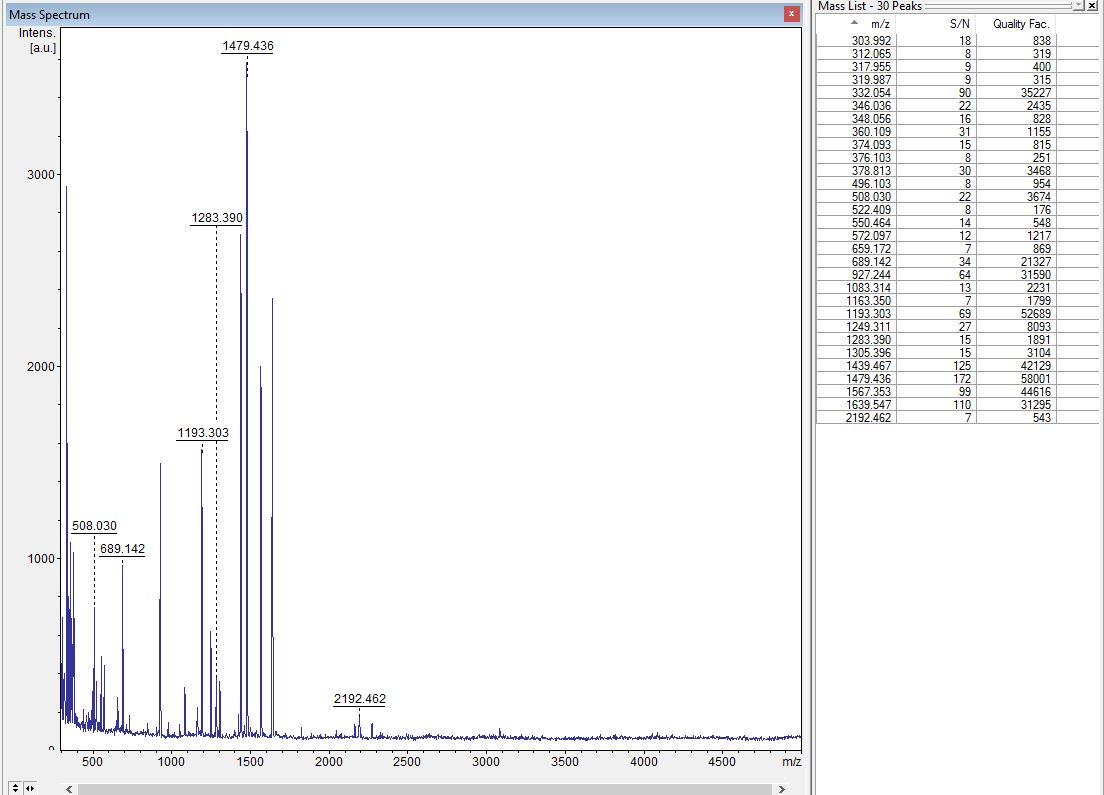
\includegraphics[width = 0.9\linewidth]{DATA.png}% Here is how to import EPS art
	\caption{\label{fig:DATA}Measured Mass Spectrum}
\end{figure}

Hemoglobin, lysozyme, BSA, ovalbumin각각의 amino sequence를 트립신을 이용해 분해한 후 나타나는 amino acid sequence와 그에 해당하는 질량 전하비는 각각 Tabs.\ref{tab:hemoglobin}, \ref{tab:lysozyme}, \ref{tab:BSA}, \ref{tab:ovalbumin} 와 같다.[1][2][3][4]

\begin{table}[h]
\caption{\label{tab:hemoglobin} hemoglobin amino acid sqeuence}
\begin{tabular}{l|c} \hline \hline
amino sequence & m/z \\ \hline
K & 146.09\\
VK & 263.16\\
AHGK & 465.19\\
HLDDLK & 829.37\\
ATITSLWGK & 1119.50\\
VHFTEEDK & 1129.45\\
VLTSLGDAIK & 1177.55\\
LHVDPENFK & 1241.53\\
MVTGVASALSSR & 1375.58\\
LLVVYPWTQR & 1435.70\\
VNVEDAGGETLGR & 1531.56\\
EFTPEVQASWQK & 1646.68\\
GTFAQLSELHCDK & 1663.64\\
LLGNVLVTVLAIHFGK & 1962.96\\
FFDSFGNLSSASAIMGNPK & 2312.86\\  \hline \hline 
\end{tabular}
\end{table}

\begin{table}[h]
\caption{\label{tab:lysozyme} lysozyme amino acid sqeuence}
\begin{tabular}{l|c} \hline \hline
amino sequence & m/z \\ \hline
R & 174.10\\
R & 174.10\\
MK & 295.13\\
NR & 306.14\\
TLK & 396.22\\
VVR & 408.24\\
DVR & 424.20\\
CQNR & 573.21\\
VFER & 603.28\\
CELAR & 662.27\\
DPQGIR & 774.32\\
AWVAWR & 877.41\\
LGMDGYR & 918.31\\
YWCNDGK & 992.31\\
ATNYNAGDR & 1124.40\\
WESGYNTR & 1137.40\\
GISLANWMCLAK & 1503.61\\
STDYGIFQINSR & 1597.63\\
ALIVLGLVLLSVTVQGK & 2010.03\\
TPGAVNACHLSCSALLQDNIADAVACAK & 3241.28\\  \hline \hline 
\end{tabular}
\end{table}

\begin{longtable}{l|c}
\caption{\label{tab:BSA} BSA amino acid sqeuence}\\
\hline \hline
amino sequence & m/z \\ \hline
\endhead
K & 146.09\\
K & 146.09\\
K & 146.09\\
K & 146.09\\
R & 174.10\\
R & 174.10\\
R & 174.10\\
R & 174.10\\
R & 174.10\\
PK & 261.14\\
LK & 277.17\\
LK & 277.17\\
HK & 301.15\\
FK & 311.16\\
QR & 320.16\\
ER & 321.14\\
YK & 327.15\\
ATK & 354.18\\
LAK & 366.21\\
VTK & 382.21\\
CCK & 388.11\\
CCK & 388.11\\
AHK & 390.19\\
AFK & 400.20\\
LVR & 422.25\\
QIK & 423.23\\
FPK & 426.21\\
VGSK & 443.19\\
YTK & 446.20\\
NLGK & 484.21\\
DEGK & 501.16\\
ADDK & 501.19\\
DVCK & 517.20\\
ASSAK & 534.23\\
LSQR & 556.27\\
FGER & 561.21\\
EQLK & 570.27\\
ADLAK & 588.28\\
HPEAK & 652.28\\
PLLEK & 670.34\\
ECCEK & 682.19\\
LDELR & 716.33\\
QEPER & 729.29\\
CASLQK & 738.31\\
AWAVAR & 762.37\\
TPVSDR & 763.33\\
NYAEAK & 784.31\\
SEVAHR & 787.34\\
AACLLPK & 822.39\\
VFDEFK & 873.37\\
LVTDLTK & 896.45\\
LCTVATLR & 1001.48\\
AEFAEVSK & 1005.42\\
YLYEIAR & 1034.46\\
DDNPNLPR & 1065.42\\
DLGEENFK & 1076.39\\
FQNALLVR & 1085.54\\
TYETTLEK & 1109.46\\
NECFLQHK & 1143.45\\
QTALVELVK & 1143.58\\
ETCFAEEGK & 1156.38\\
SLHTLFGDK & 1160.49\\
CCTESLVNR & 1167.43\\
LVNEVTEFAK & 1310.59\\
AAFTECCQAADK & 1454.52\\
PLVEEPQNLIK & 1458.68\\
HPDYSVVLLLR & 1490.71\\
ETYGEMADCCAK & 1517.45\\
AVMDDFAAFVEK & 1539.63\\
YICENQDSISSK & 1583.58\\
CCAAADPHECYAK & 1596.52\\
TCVADESAENCDK & 1599.52\\
VPQVSTPTLVEVSR & 1744.82\\
QNCELFEQLGEYK & 1815.67\\
DVFLGMFLYEYAR & 1838.74\\
PCFSALEVDETYVPK & 1948.78\\
HPYFYAPELLFFAK & 1975.86\\
VHTECCHGDLLECADDR & 2202.74\\
EFNAETFTFHADICTLSEK & 2525.98\\
PEVDVMCTAFHDNEETFLK & 2547.97\\
MPCAEDYLSVVLNQLCVLHEK & 2763.13\\
ALVLIAFAQYLQQCPFEDHVK & 2792.24\\
SHCIAEVENDEMPADLPSLAADFVESK & 3384.29\\  \hline \hline 
\end{longtable}

\begin{table}[h]
\caption{\label{tab:ovalbumin} ovalbumin amino acid sqeuence}
\begin{tabular}{l|c} \hline \hline
amino sequence & m/z \\ \hline
K & 146.09\\
IK & 277.17\\
MK & 295.13\\
MK & 295.13\\
AFK & 400.20\\
VVR & 408.24\\
ELK & 424.21\\
FDK & 444.19\\
DSTR & 531.21\\
MEEK & 589.21\\
ELYR & 633.28\\
TQINK & 674.32\\
GLWEK & 703.29\\
VYLPR & 718.36\\
LYAEER & 869.36\\
VTEQESK & 927.38\\
VASMASEK & 947.38\\
DILNQITK & 1069.51\\
ADHPFLFCIK & 1351.58\\
DEDTQAMPFR & 1370.51\\
HIATNAVLFFGR & 1542.70\\
PNDVYSFSLASR & 1552.63\\
YPILPEYLQCVK & 1662.73\\
PVQMMYQIGLFR & 1679.71\\
LTEWTSSNVMEER & 1796.69\\
GGLEPINFQTAADQAR & 1956.78\\
GSIGAASMEFCFDVFK & 1977.71\\
ISQAVHAAHAEINEAGR & 2060.86\\
ELINSWVESQTNGIIR & 2127.90\\
EVVGSAEAGVDAASVSEEFR & 2349.89\\
LPGFGDSIEAQCGTSVNVHSSLR & 2769.05\\
NVLQPSSVDSQTAMVLVNAIVFK & 2855.29\\
VHHANENIFYCPIAIMSALAMVYLGAK & 3443.43\\
YNLTSVLMAMGITDVF & \multirowcell{2}{3850.53}\\
SSSANLSGISSAESLK & \\
ILELPFASGTMSMLVLL & \multirowcell{2}{4473.89}\\  
PDEVSGLEQLESIINFEK & \\ \hline \hline 
\end{tabular}
\end{table}


Fig.\ref{fig:DATA}에서 측정된 피크값에 대해서 최소의 차이를 가지는 sequence를 구한 후 그 차이를 퍼센트로 나타내면 Fig.\ref{tab:cov}와 같다. 단, 가속되는 전하가 $[\ch{MH}^{+}]$이므로 각 mass spectrum에서 양성자의 질량을 제외하였다. Coverage의 경우 차이의 절대값이 $2.5\%$이하인 경우 amino acid sequence를 잘 설명한다고 가정하였으며 이를 통해 amino acid sequence를 잘 설명하는 비율을 coverage로 계산하였다. BSA가 $90\%$의 coverage로 가장 높은 값을 가지므로 주어진 단백질은 BSA라고 할 수 있다.

\begin{table}[]
\caption{\label{tab:cov} Measured Coverage}
\begin{tabular}{c|c|c|c|c} \hline \hline
m/z & hemoglobin & lysozyme & BSA & ovalbumin \\ \hline
302.99 & 13.15\% &-1.04\% &0.61\% &2.59\%\\
311.06 & 15.40\% &1.58\% &-0.03\% &5.12\%\\
316.95 & 16.97\% &3.41\% &-1.01\% &6.89\%\\
318.99 & 17.50\% &4.03\% &-0.37\% &7.48\%\\
331.05 & 20.51\% &7.53\% &1.18\% &10.85\%\\
345.04 & 23.73\% &11.27\% &-2.65\% &14.46\%\\
347.06 & 24.17\% &11.79\% &-2.05\% &14.96\%\\
359.11 & 26.72\% &-10.33\% &1.37\% &-11.44\%\\
373.09 & -24.68\% &-6.20\% &1.84\% &-7.27\%\\
375.10 & -24.02\% &-5.63\% &-1.89\% &-6.69\%\\
377.81 & -23.13\% &-4.87\% &-1.16\% &-5.93\%\\
495.10 & 6.04\% &14.32\% &-1.22\% &-7.29\%\\
507.03 & 8.25\% &-13.05\% &1.15\% &-4.77\%\\
521.41 & 10.78\% &-9.93\% &0.81\% &-1.88\%\\
549.46 & 15.34\% &-4.32\% &-1.24\% &3.32\%\\
571.10 & 18.54\% &-0.37\% &0.14\% &-3.17\%\\
658.17 & -26.01\% &-0.62\% &0.90\% &-2.45\%\\
688.14 & -20.52\% &3.76\% &0.86\% &2.01\%\\
926.24 & 10.46\% &0.86\% &3.22\% &-0.12\%\\
1082.31 & -3.44\% &-3.89\% &-0.30\% &1.18\%\\
1162.35 & -1.31\% &2.15\% &0.16\% &7.99\%\\
1192.30 & 1.24\% &4.60\% &2.09\% &10.30\%\\
1248.31 & 0.54\% &8.88\% &-4.99\% &-8.27\%\\
1282.39 & 3.19\% &11.31\% &-2.20\% &-5.40\%\\
1304.40 & 4.82\% &12.80\% &-0.47\% &-3.62\%\\
1438.47 & 0.19\% &-4.53\% &-1.12\% &4.72\%\\
1478.44 & 2.89\% &-1.70\% &-0.83\% &-4.35\%\\
1566.35 & 2.22\% &-2.00\% &-1.10\% &0.88\%\\
1638.55 & -0.50\% &2.50\% &2.38\% &-1.48\%\\
2191.46 & -5.54\% &8.28\% &-0.51\% &2.90\%\\ \hline
coverage & 20.00\% & 30.00\% & 90.00\% & 23.33\% \\  \hline \hline 
\end{tabular}
\end{table}


\section{\label{sec:level1}Discussion \& Conclusion}
실험 결과 대부분의 amino acid가 BSA를 통해 설명이 되고 약 $90\%$의 coverage를 가져 높은 확률로 주어진 단백질은 BSA일 것이다. m/z값 1248.31을 가지는 amino acid의 경우 약 $4.99\%$의 오차를 가지는데 해당 amino acid에서 miscleavage가 발생하여 나타난 peak라고 결론지었다. 하지만 BSA의 높은 m/z에 해당하는 amino acid는 peak로 나타나지 않았다. 이것은 주어진 load에서 레이저를 가하는 부분에 따라 나타나는 peak가 달라지므로 load의 여러부분에 레이저를 인가하고 평균값을 취하는 경우 높은 m/z에 해당하는 peak를 확인할 수 있을 것이다. 또한 본 실험에서 어떤 단백질을 이용하는지에 따라 coverage값이 달라진다. 예를 들어 본 보고서에서는 사람으로부터 추출된 hemoglobin을 이용해 데이터를 분석하였다. 하지만 개부터 주어지는 hemoglobin의 amino acid sequence는 공통적인 부분을 가지기도 하나 다른 서열이 나타나기도 하여 약 33\%의 coverage를 가진다.[7] 따라서 주어진 단백질이 어떤 생물체로부터 주어졌는지 등 부가적인 조건이 있는 경우 더 정확한 단백질 동정이 가능할 것이다. 그리고 miscleavage를 방지하기 위해 더 오랜 시간 단백질을 변성시키고, 더 오랜 시간 트립신과 반응시키는 경우 더 정확한 실험 결과를 얻을 수 있을 것이다.

\section{\label{sec:level1}Reference}
[1] Bank, R. P. D. (n.d.). \textit{1D PFV: 4MQJ}. https://www.rcsb.org/sequence/4MQJ

[2] \textit{UniProt}. (n.d.). https://www.uniprot.org/uniprotkb/ P61626/entry\#sequences

[3] Bank, R. P. D. (n.d.). \textit{3D View: 7JWN}. https://www.rcsb.org/3d-view/7JWN

[4] Bank, R. P. D. (n.d.). \textit{3D View: 1UHG}. https://www.rcsb.org/3d-view/1UHG

[5] Garrett, R. H., \& Grisham, C. M. (2002, January 1). The Primary Structure of a Protein: Determining the Amino Acid Sequence. In \textit{Principles of Biochemistry} (pp. 134-135). Cengage Learning.

[6] Garrett, R. H., \& Grisham, C. M. (2002, January 1). Mechanisms of Enzyme Action. In \textit{Principles of Biochemistry} (pp. 514-515). Cengage Learning.

[7] Bank, R. P. D. (n.d.). \textit{RCSB PDB - 3GOU: Crystal structure of dog (Canis familiaris) hemoglobin}. https://www.rcsb.org/structure/3GOU


\end{document}
%
% ****** End of file apssamp.tex ******
